\section{Transport}
\label{sec:transport}

\label{describe_transport}

To transport sea ice fractional area and various tracers, MPAS-Seaice uses an incremental remapping (IR) algorithm similar to that described by \citet{Dukowicz00}, \citet{Lipscomb04} (henceforth LH04) and \citet{Lipscomb05} (henceforth LR05). The LH04 scheme was designed for structured quadrilateral meshes and is implemented in CICE \citep{Hunke15}. The LR05 scheme was implemented on a structured SCVT global mesh consisting of quasi-regular hexagons and 12 pentagons.

For MPAS-Seaice the IR scheme was generalized to work on either the standard MPAS mesh (hexagons and other n-gons of varying sizes, with a vertex degree of 3 as in LR05) or a quadrilateral mesh (with a vertex degree of 4 as in LH04 and CICE). Since MPAS meshes are unstructured, the IR scheme had to be rewritten from scratch. Most of the code is mesh-agnostic, but a small amount of code is specific to quad meshes as noted below.

Here we review the conceptual framework of incremental remapping as in \citep{Hunke15} and describe features specific to the MPAS-Seaice implementation. IR is designed to solve equations of the form
\begin{equation}
\label{eq:transport_m}
\frac{\partial m}{\partial t} =-\nabla \boldsymbol{\cdot} (\mathbf{u}m)
\end{equation}
\begin{equation}
\label{eq:transport_T1}
\frac{\partial (m T_1)}{\partial t} = -\nabla \boldsymbol{\cdot} (\mathbf{u} m T_1),
\end{equation}
\begin{equation}
\label{eq:transport_T2}
\frac{\partial (m T_1 T_2)}{\partial t} = -\nabla \boldsymbol{\cdot} (\mathbf{u} m T_1 T_2),
\end{equation}
\begin{equation}
\label{eq:transport_T3}
\frac{\partial (m T_1 T_2 T_3)}{\partial t} = -\nabla \boldsymbol{\cdot} (\mathbf{u} m T_1 T_2 T_3),
\end{equation}
where $\mathbf{u} = (x,y)$ is the horizontal velocity, $m$ is mass or a mass-like field (such as density or fractional sea ice concentration), and $T_1$, $T_2$ and $T_3$ are tracers.  These equations describe conservation of quantities such as mass and internal energy under horizontal transport. Sources and sinks of mass and tracers (e.g., ice growth and melting) are treated separately from transport.  

In MPAS-Seaice, the fractional ice area in each thickness category is a mass-like field whose transport is described by (\ref{eq:transport_m}). (Henceforth, ``area'' refers to fractional ice area unless stated otherwise.) Ice and snow thickness, among other fields, are type 1 tracers obeying equations of the form (\ref{eq:transport_T1}), and the ice and snow enthalpy in each vertical layer are type 2 tracers obeying equations like (\ref{eq:transport_T2}), with ice or snow thickness as their parent tracer. When run with advanced options (e.g., active melt ponds and biogeochemistry), MPAS-Seaice advects tracers up to type 3. Thus, the mass-like field is the ``parent field'' for type 1 tracers; type 1 tracers are parents of type 2; and type 2 tracers are parents of type 3.

Incremental remapping has several desirable properties for sea ice modeling:
\begin{itemize}
\item It is conservative to within machine roundoff.
\item It preserves tracer monotonicity.  That is, transport produces no new local extrema in fields like ice thickness or internal energy. 
\item The reconstructed mass and tracer fields vary linearly in x and y. This means that remapping is second-order accurate in space, except where gradients are limited locally to preserve monotonicity.
\item There are economies of scale.  Transporting a single field is fairly expensive, but additional tracers have a low marginal cost, especially when all tracers are transported with a single velocity field as in CICE and MPAS-Seaice.
\end{itemize}

The time step is limited by the requirement that trajectories projected backward from vertices are confined to the cells sharing the vertex (i.e., 3 cells for the standard MPAS mesh and 4 for the quad mesh).  This is what is meant by incremental as opposed to general remapping. This requirement leads to a CFL-like condition,
\begin{equation}
\label{eq:IR_CFL}
\frac{\max (|\mathbf{u}|\Delta t)}{\Delta x}\le 1,
\end{equation}
where $\Delta x$ is the grid spacing and $\Delta t$ is the time step. For highly divergent velocity fields, the maximum time step may have to be reduced by a factor of 2 to ensure that trajectories do not cross. 

The IR algorithm consists of the following steps:
\begin{itemize}
\item Given mean values of the ice area and tracer fields in each grid cell and thickness category, construct linear approximations of these fields. Limit the field gradients to preserve monotonicity.
\item Given ice velocities at grid cell vertices, identify departure regions for the transport across each cell edge. Divide these departure regions into triangles and compute the coordinates of the triangle vertices.
\item Integrate the area and tracer fields over the departure triangles to obtain the area, volume, and other conserved quantities transported across each cell edge.
\item Given these transports, update the area and tracers.
\end{itemize}
\noindent
Since all fields are transported by the same velocity field, the second step is done only once per time step. The other steps are repeated for each field.

With advanced physics and biogeochemistry (BGC) options, MPAS-Seaice can be configured to include up to $\sim$40 tracer fields, each of which is advected in every thickness category, and many of which are defined in each vertical ice or snow layer. In order to accommodate different tracer combinations and make it easy to add new tracers, the tracer fields are organized in a linked list that depends on which physics and BGC packages are active. The list is arranged with fractional ice area first, followed by the type 1 tracers, type 2 tracers, and finally type 3 tracers. In this way, values computed for parent tracers are always available when needed for computations involving child tracers.

We next describe the IR algorithm in detail, pointing out features that are new in MPAS-Seaice.

\subsubsection{Reconstructing area and tracer fields}
\label{IR_reconstruct}

The fractional ice area and all tracers are reconstructed in each grid cell (quadilaterals, hexagons or other $n$-gons) as functions of $\mathbf{r} = (x,y)$ in a cell-based coordinate system. On a sphere, $\mathbf{r}$ lies in a local plane that is tangent to the sphere at the cell center. The state variable for ice area, denoted as $\bar{a}$, should be recovered as the mean value when integrated over the cell:
\begin{equation}
\label{eq:recover_a}
\int_{A}{a(x,y)dA=\bar{a}{{A}_{C}}},
\end{equation}
where $A_C$ is the grid cell area. Equation~\ref{eq:recover_a} is satisfied if $a(\mathbf{r})$ has the form
\begin{equation}
\label{eq:reconstruct_a}
a(\mathbf{r})=\bar{a}+{{\alpha }_{a}}\nabla a \boldsymbol{\cdot} (\mathbf{r}-\mathbf{\bar{r}}),
\end{equation}
where $\nabla a$ is a cell-centered gradient, ${\alpha }_{a}$ is a coefficient between 0 and 1 that enforces monotonicity, and $\mathbf{r}$ is the cell centroid:
\begin{equation}
\label{eq:centroid}
\mathbf{\bar{r}}=\frac{1}{{{A}_{C}}}\int_{A}{\mathbf{r} dA}.
\end{equation}
Similarly, tracer means should be recovered when integrated over a cell:
\begin{align}
\begin{split} % so there will be only one equation number
\label{eq:recover_T}
   \int_{A}{a(\mathbf{r}){{T}_{1}}}(\mathbf{r})dA & = \bar{a}{{{\bar{T}}}_{1}}{{A}_{C}},  \\
   \int_{A}{a(\mathbf{r}){{T}_{1}}}(\mathbf{r}){{T}_{2}}(\mathbf{r})dA & =\bar{a}{{{\bar{T}}}_{1}}{{{\bar{T}}}_{2}}{{A}_{C}},  \\
   \int_{A}{a(\mathbf{r}){{T}_{1}}}(\mathbf{r}){{T}_{2}}(\mathbf{r}){{T}_{3}}(\mathbf{r})dA & = \bar{a}{{{\bar{T}}}_{1}}{{{\bar{T}}}_{2}}{{{\bar{T}}}_{3}}{{A}_{C}}.
\end{split}
\end{align}
These equations are satisfied when the tracers are reconstructed as
\begin{align}
\begin{split}
\label{eq:reconstruct_T}
   {{T}_{1}}(\mathbf{r}) = {{{\bar{T}}}_{1}}+{{\alpha }_{T1}}\nabla {{T}_{1}}\cdot (\mathbf{r}-{{{\mathbf{\tilde{r}}}}_{1}}),  \\
   {{T}_{2}}(\mathbf{r}) = {{{\bar{T}}}_{2}}+{{\alpha }_{T2}}\nabla {{T}_{2}}\cdot (\mathbf{r}-{{{\mathbf{\tilde{r}}}}_{2}}),  \\
   {{T}_{3}}(\mathbf{r}) = {{{\bar{T}}}_{3}}+{{\alpha }_{T3}}\nabla {{T}_{3}}\cdot (\mathbf{r}-{{{\mathbf{\tilde{r}}}}_{3}}),
\end{split}
\end{align}
where the tracer barycenter coordinates $\mathbf{\tilde{r}}_n$ are given by
\begin{align}
\begin{split}
\label{eq:barycenters}
   {{{\mathbf{\tilde{r}}}}_{1}} & = \frac{1}{\bar{a}{{A}_{C}}}\int_{A}{\mathbf{r}adA,}  \\
   {{{\mathbf{\tilde{r}}}}_{2}} & = \frac{1}{\bar{a}{{{\bar{T}}}_{1}}{{A}_{C}}}\int_{A}{\mathbf{r}a{{T}_{1}}dA,}  \\
   {{{\mathbf{\tilde{r}}}}_{3}} & = \frac{1}{\bar{a}{{{\bar{T}}}_{1}}{{{\bar{T}}}_{2}}{{A}_{C}}}\int_{A}{\mathbf{r}a{{T}_{1}}{{T}_{2}}dA.}
\end{split}
\end{align}
The integrals in (\ref{eq:barycenters}) can be evaluated by applying quadrature rules for linear, quadratic and cubic polynomials as described in Section~\ref{IR_integrate}.

Monotonicity is enforced by van Leer limiting \citep{vanLeer79}. The reconstructed area and tracers are evaluated at cell vertices, and the coefficients $\alpha$  are reduced as needed so that the reconstructed values lie within the range of the mean values in the cell and its neighbors. When $\alpha = 1$, the reconstruction is second-order accurate in space. When $\alpha = 0$, the reconstruction reduces locally to first-order.

\subsubsection{Locating departure triangles}
\label{IR_triangles}

The next step is to identify the departure region associated with fluxes across each cell edge, and to divide the departure region into triangles. Figure~\ref{fig:IR_geom}a illustrates the geometry for the standard MPAS mesh. The edge has vertices $V1$ and $V2$. Each edge is oriented such that one adjacent cell ($C1$) is defined to lie in the left half-plane and the other ($C2$) in the right half-plane. The departure points $D1$ and $D2$ are found by projecting velocities backward from $V1$ and $V2$. The shaded departure region is a quadrilateral containing all the ice transported across the edge in one time step. In addition to $C1$ and $C2$, the departure region can include side cells $C3$ and $C4$. The side cells share edges $E1$ to $E4$ and vertices $V3$ to $V6$ with the central cells $C1$ and $C2$.

\begin{figure}[]
\centering
%\includegraphics[width=0.6\textwidth]{IRhex.pdf}
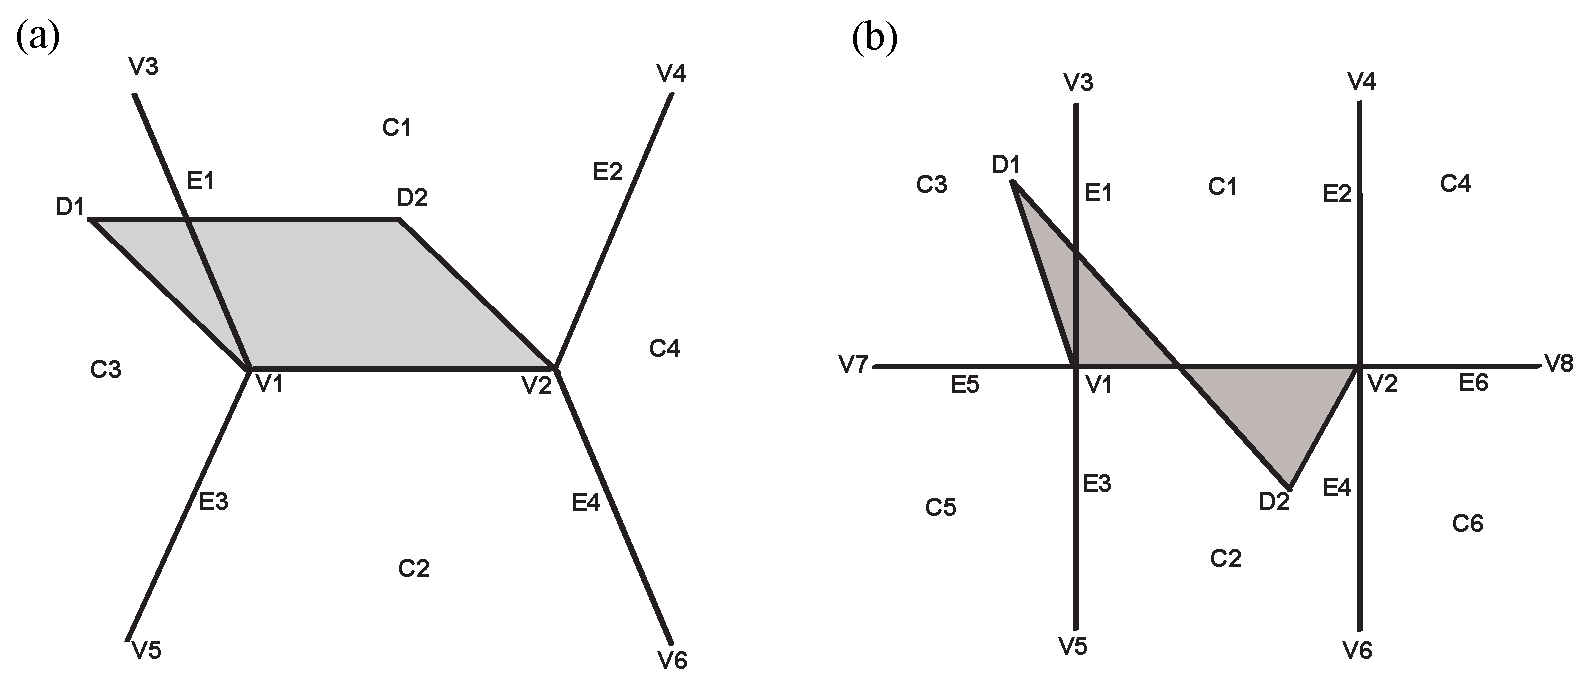
\includegraphics[width=1.0\textwidth]{seaice/ir_diagram.eps}
\caption{(a): Schematic showing transport across a cell edge on a standard MPAS mesh with 3 edges meeting at each vertex. The letters $C$, $E$ and $V$ denote cell centers, edges and vertices, respectively. Points $D1$ and $D2$ are backward trajectories, and the departure region is shaded. (b): Schematic showing transport across a cell edge on a quadrilateral MPAS mesh with 4 edges meeting at each vertex.}
\label{fig:IR_geom}
\end{figure}

The edges and vertices in Figure~\ref{fig:IR_geom}a are defined in a coordinate system lying in the local tangent plane at the midpoint of the main edge, halfway between $V1$ and $V2$. These coordinates are pre-computed at initialization. During each time step, departure triangles are found by locating $D1$ and $D2$ in this coordinate system, and then looping through the edges to identify any intersections of line segment $\overline{D12}$ (i.e., the segment joining $D1$ and $D2$) with the various edges. If $\overline{D12}$ intersects the main edge, then the departure region consists of two triangles (one each in $C1$ and $C2$) rather than a quadrilateral (as shown in the figure). If $\overline{D12}$ intersects any of edges $E1$ to $E4$, the departure region includes triangles in side cells.

Each departure triangle lies in a single grid cell, and there are at most four such triangles. There are two triangles in the central cells (either one each in $C1$ and $C2$, or a quadrilateral that can be split into two triangles), and up to two triangles in side cells. The triangle vertices are a combination of cell vertices ($V1$ and $V2$), departure points ($D1$ and $D2$), and intersection points (points where $\overline{D12}$ crosses an edge).

Figure~\ref{fig:IR_geom}b shows the geometry for a quadrilateral mesh. In this figure the departure region consists of two triangles, but it could also be a quadrilateral as in Figure~\ref{fig:IR_geom}a. For the quad mesh there are two additional side cells ($C5$ and $C6$), edges ($E5$ and $E6$) and vertices ($V7$ and $V8$). The search algorithm is designed such that the code used to find departure triangles for the standard mesh is also  applied to the quad mesh. For quad meshes only, there is additional logic to find intersection points and triangles associated with the extra edges and cells. This is the only mesh-specific code in the run-time IR code. For the quad mesh there are at most six departure triangles: two in the central cells and one in each of the four side cells. If the edges meet at right angles as shown in the figure, the maximum is five triangles, but this is not a mesh requirement.

Once triangle vertices have been found in edge-based coordinates, they are transformed to cell-based coordinates, i.e., coordinates in the local tangent plane of the cell containing each triangle. (Coefficients for these transformations are computed at initialization.) Triangle areas are computed as 
\begin{equation}
\label{eq:triangle_area}
{{A}_{T}}=\frac{1}{2}\left| ({{x}_{2}}-{{x}_{1}})({{y}_{3}}-{{y}_{1}})-({{y}_{2}}-{{y}_{1}})({{x}_{3}}-{{x}_{1}}) \right|.
\end{equation}

\subsubsection{Integrating the transport}
\label{IR_integrate}

Next, ice area and area-tracer products are integrated in each triangle. The integrals have the form (\ref{eq:recover_a}) for area and (\ref{eq:recover_T}) for tracers. Since each field is a linear function of $(x,y)$ as in (\ref{eq:reconstruct_a}) and (\ref{eq:reconstruct_T}), the area-tracer products are quadratic, cubic and quartic polynomials, respectively, for tracers of type 1, 2 and 3.

The integrals can be evaluated exactly by summing over values at quadrature points in each triangle. Polynomials of quadratic or lower order are integrated using the formula
\begin{equation}
\label{eq:quadrature1}
I = \frac{{{A}_{T}}}{3}\sum\limits_{i=1}^{3}{f({{{\mathbf{{x}'}}}_{i}})}.
\end{equation}
The quadrature points are located at ${{\mathbf{{x}'}}_{i}}=({{\mathbf{x}}_{0}}+{{\mathbf{x}}_{i}})/2$, where $\mathbf{x_0}$ is the triangle midpoint and $\mathbf{x_i}$ are the three vertices. The products involving type-2 and type-3 tracers are cubic and quadratic polynomials, which can be evaluated using a similar formula with 6 quadrature points:
\begin{equation}
\label{eq:quadrature2}
I = {{A}_{T}}\left[ {{w}_{1}}\sum\limits_{i=1}^{3}{f({{\mathbf{x}}_{1i}})}+{{w}_{2}}\sum\limits_{i=1}^{3}{f({{\mathbf{x}}_{2i}})} \right],
\end{equation}
where $\mathbf{x_{1i}}$ and $\mathbf{x_{2i}}$ are two sets of three quadrature points, arranged symmetrically on trisecting medians of the triangle, and $w_1$ and $w_2$ are weighting factors. Coefficients and weighting factors for these and other symmetric quadrature rules for triangles were computed by \citet{Dunavant85}. These integrals are computed for each triangle and summed over edges to give fluxes of ice area and area-tracer products across each edge.

\subsubsection{Updating area and tracer fields}
\label{IR_update}

The area transported across edge $k$ for a given cell can be denoted as $\Delta a_k$,  and the area-tracer products as $\Delta (a T_1)_k$, $\Delta (a T_1 T_2)_k$ and $\Delta (a T_1 T_2 T_3)_k$. The new ice area at time $n+1$ is given by
\begin{equation}
\label{eq:update_a}
{{a}^{n+1}} = {{a}^{n}}+\frac{1}{{{A}_{C}}}\sum\limits_{k}{\pm \Delta {{a}_{k}}},
\end{equation}
where the sum is taken over cell edges $k$, with a positive sign denoting transport into a cell and a negative sign denoting outward transport. The new tracers are given by
\begin{align}
\begin{split}
\label{eq:update_T}
   T_{1}^{n+1} & = \frac{{{a}^{n}}T_{1}^{n}+\frac{1}{{{A}_{C}}}\sum\limits_{k}{\pm \Delta {{(a{{T}_{1}})}_{k}}}}{{{a}^{n+1}}},  \\
   T_{2}^{n+1} & = \frac{{{a}^{n}}T_{1}^{n}T_{2}^{n}+\frac{1}{{{A}_{C}}}\sum\limits_{k}{\pm \Delta {{(a{{T}_{1}}{{T}_{2}})}_{k}}}}{{{a}^{n+1}}T_{1}^{n+1}},  \\
   T_{3}^{n+1} & =\frac{{{a}^{n}}T_{1}^{n}T_{2}^{n}T_{3}^{n}+\frac{1}{{{A}_{C}}}\sum\limits_{k}{\pm \Delta {{(a{{T}_{1}}{{T}_{2}}{{T}_{3}})}_{k}}}}{{{a}^{n+1}}T_{1}^{n+1}T_{2}^{n+1}}.
\end{split}
\end{align}
\citet{Dukowicz00} showed that (\ref{eq:update_T}) satisfies tracer
monotonicity, since the new-time tracer values are area-weighted
averages of old-time values.

